% +--------------------------------------------------------------------+
% | Sample Chapter 2
% +--------------------------------------------------------------------+

\cleardoublepage

% +--------------------------------------------------------------------+
% | Replace "This is Chapter 2" below with the title of your chapter.
% | LaTeX will automatically number the chapters.
% +--------------------------------------------------------------------+

\chapter{State of the Art}
\label{makereference2}

This chapter describes the current state of Edge computing related to Internet of Things. Different types of architectures that diverge in core technologies regarding edge environments are going to be discussed,  also we'll cover some projects that provide \textit{similar} solutions to Epfiot.

Chapter ~\ref{makereference} has covered some basic definitions used in the project such as Virtualization, however this is not the only option regarding technologies that allows to prepare the proper infrastructure in a edge context.

\section{Containers, lightweight alternative}
\label{makereference2.1}

Virtualization has been around for a long time but since a few years ago, containers were adopted globally, transforming the IT world
as we currently know it.

A \textbf{Container} is a set of one or more process that are isolated from the rest of the operating system. These process would lately be very useful to prepare independent components that share resources with the host machine and have portability. 
Containers are a form of virtualization, while virtualization works at hardware level emulating all the resources that are needed for a guest operating system to run. Containers, in the other hand work at operating system level being a lightweight alternative.

The idea of the container technology first appeared in 2000 as FreeBSD jail, safe environment that a system administrator could share with multiple users. Later on more technologies were combined to become this isolated approach a reality. For example Control groups is a kernel feature that monitors and limits resource usage for a process or groups of processes or Systemd, an initialization system that sets up the userspace and manages their processes. In 2008 Docker was born with a new container technology adding new concepts and tools, layered images, command line tools, a server daemon granting, granting to the user the ability of build new containers quickly and share between others.~\cite{redhat_container}

\begin{figure}[h!]%t=top, b=bottom, h=here
    \centering
    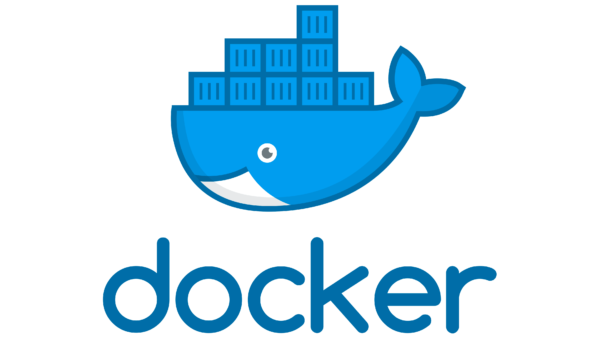
\includegraphics[width=2.5in]{figures/docker.png}
~\caption{docker container logo}
\label{figure2.1}
\end{figure}

\section{Virtualization and Containers, what to choose}
\label{makereference2.2}

The infrastructure takes into account several factors.

\begin{itemize}
    \item System software that is going to run at the top of the architecture fast and lightweight. Designed to operate directly on edge devices (computation, network, storage) and for this purpose, normally system software needs the support of multi-tenancy and isolation.
    \item Resource constrained because edge devices have smaller processors and limited power budget ~\ref{makereference1.1}. Managing these resources properly is one of the challenge that edge computing needs to confront.
    \item Elastic escalation, depending on the services that are going to be provided.
    \item Network capabilities
\end{itemize}
Usually, in an edge computing scenario, several applications are running from different tenants. Due to the factors previously discussed, both containers and virtual machines are valid approaches in order to satisfy the edge requirements.~\cite{CORR:chong:2018} Both enable fault and performance isolation between tenants and limits the accounts for the resource usage.
\newpage

However there are differences, see figure \ref{figure2.2}.

\begin{itemize}
  \item Virtual Machines are built including virtualized resources that emulate the entire computer such as  CPU, memory, network, storage, gpu... This means that the tenant installs the operating system and runs applications like in a real physical machine. Virtualization isolates completely the execution environment.
  \item Containers are lightweight virtualization and are multiplexed by a single Linux kernel. They don't require an additional layer if you compare them with the virtual machines. They share the same OS kernel, keeping the isolation principles by using cgroups and Linux namespaces. This allows the containers to achieve performance similar to the native environment.
\end{itemize}

\begin{figure}[h]%t=top, b=bottom, h=here
% \centering
    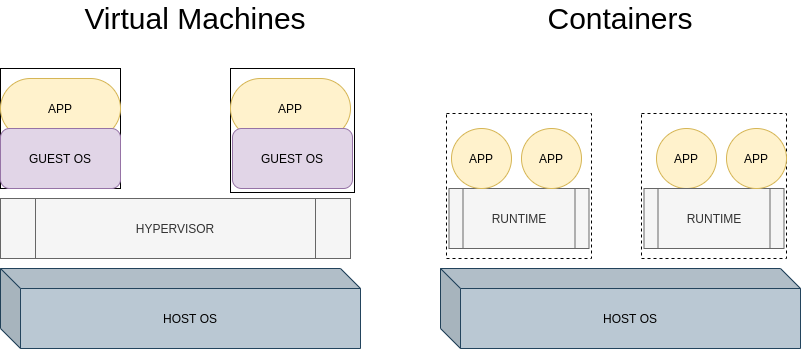
\includegraphics[width=6.5in]{figures/virt_container.png}
~\caption{virtual machine architecture and container architecture}
\label{figure2.2}
\end{figure}

To choose what kind of technology is better in a edge environment is not an easy question. Virtualization approaches varies from system to system. Many recent works chose lightweight OS-Level virtualization like LXC to run services on edge systems that have limited storage and processing capabilities. Unlike virtual machines, multiple containers share the same Linux kernel and therefore exhibit very small overhead.~\cite{ACM:clixue:2018}



Taking into account the lightweight capability of the containers reducing resource consumption it could be said that is the perfect solution for Edge computing. However it faces serious security problems that are solved in a virtual machine architecture. 

\newpage

In order to compare both technologies, a table has been provides, see table \ref{table1}.

\begin{table}
    \begin{center}
    \begin{tabular}[h]{|c|c|}
        \hline
        \textbf{Virtual Machines} & \textbf{Containers}\\
        \hline
        Heavyweight & Lightweight\\
        Each VM runs in its own OS	 & All containers share the host OS\\
        Hardware-level virtualization & OS virtualization \\
        Startup time in minutes	 & Startup time in milliseconds \\
        Allocates required memory & Requires less memory space \\
        Fully isolated and hence more secure & Process-level isolation, possibly less secure\\
        \hline
    \end{tabular}
    \caption{vms and container comparison. ~\cite{virt_comparison}}
    \label{table1}
   \end{center}
\end{table}


Security issues is one of the most important things to take into account, however containers are lightweight, have better startup time and the resource requirements are by far better considering that we are in a edge environment and all its implications. These important factors are defined in ~\ref{makereference2.2}

However EPFIOT project takes that into account and with the new forms of virtualization there are some key features that could be improved:
\begin{itemize}
    \item Baremetal performance using Linux hypervisor
    \item hardware passthrough
    \item lightweight vm images
\end{itemize}

These features balance both technologies, on an edge approach it would be better to use containers if the service requires a high level of escalation on demand and the security issues are covered. Moreover in a scenario that  this high elastic escalation is not required and some third party hardware is being used (usb accelerators), a virtualization approach would be a better fit. Taking into account that usually you need concrete hardware requirements to meet with the third party hardware provider.

\newpage

\section{Similar solutions}
\label{makereference2.3}

Projects focus in the same problem have been proposed using different perspectives. Some of them are listed below.

\subsection{Openstack for cloudlet deployments}
\label{makereference2.3.1}

Openstack ~\cite{openstack} is a cloud operating system that controls large pools of compute, storage and networking resource throughout a datacenter, managed and provisioned through APIs with authentication mechanism.
A dashboard is also available, giving administrators control while empowering their users to provision resources through a web interface. 

\begin{figure}[h]%t=top, b=bottom, h=here
% \centering
    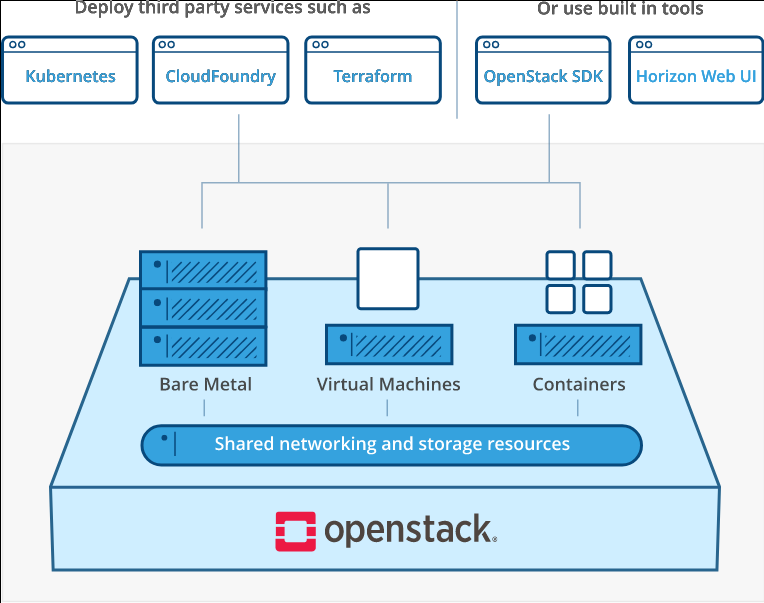
\includegraphics[width=6.0in]{figures/openstack.png}
~\caption{Openstack overview, from Openstack official page}
\label{figure2.2}
\end{figure}

\newpage

\textbf{Cloudlet} ~\cite{cloudlet_def} is a concept that emerges from the convergence of cloud computing and mobile computing, is a mobility-enhanced small-scale cloud datacenter located at the edge of the internet. Its main purpose is supporting resource-intensive and interactive mobile applications providing powerful computing resources to mobile devices with lower latency.

Openstack was built thinking in large scale IT enterprise, why is it a relevant project for Edge Computing then? Openstack is an immense open source. The programmer could create distributions following his ow needs.

Openstack++ ~\cite{Cloudlet:2015} is a distribution that extends OpenStack to leverage its open ecosystem bringing the cloudlet concept into openstack while changing the vm model with the following features:

\begin{itemize}
    \item Import Base VM: Import a Base VM from a image storage.
    \item Resume Base VM: Resume one of the base VMs to make a customized VM and to create a new VM
    \item Create VM overlay: Create a VM overlay from a running VM instance.
    \item VM synthesis: Provisioning a VM instance at a OpenStack++ cluster using a VM overlay.
    \item VM handoff: Migrating a VM instance to a different OpenStack++ cluster.
\end{itemize}

This distribution was implemented by researchers at Carnegie Mellon University.
\newpage
\subsection{OpenNebula and Telefonica Onlife}
\label{makereference2.3.2}

Opennebula is a cloud computing platform that have Openstack's similar features but relying in simplicity over a complex plugin architecture.

Telefonica is utilizing OpenNebula to prototype a new generation of Central offices that allows the deployment of programmable services rather than the traditional black box solutions. Telefónica aims to virtualize the access network and give third-party Internet of Things application developers and content providers cloud-computing capabilities at the network edge.~\cite{IEC:Opennebula:2017}

\begin{figure}[h]%t=top, b=bottom, h=here
% \centering
    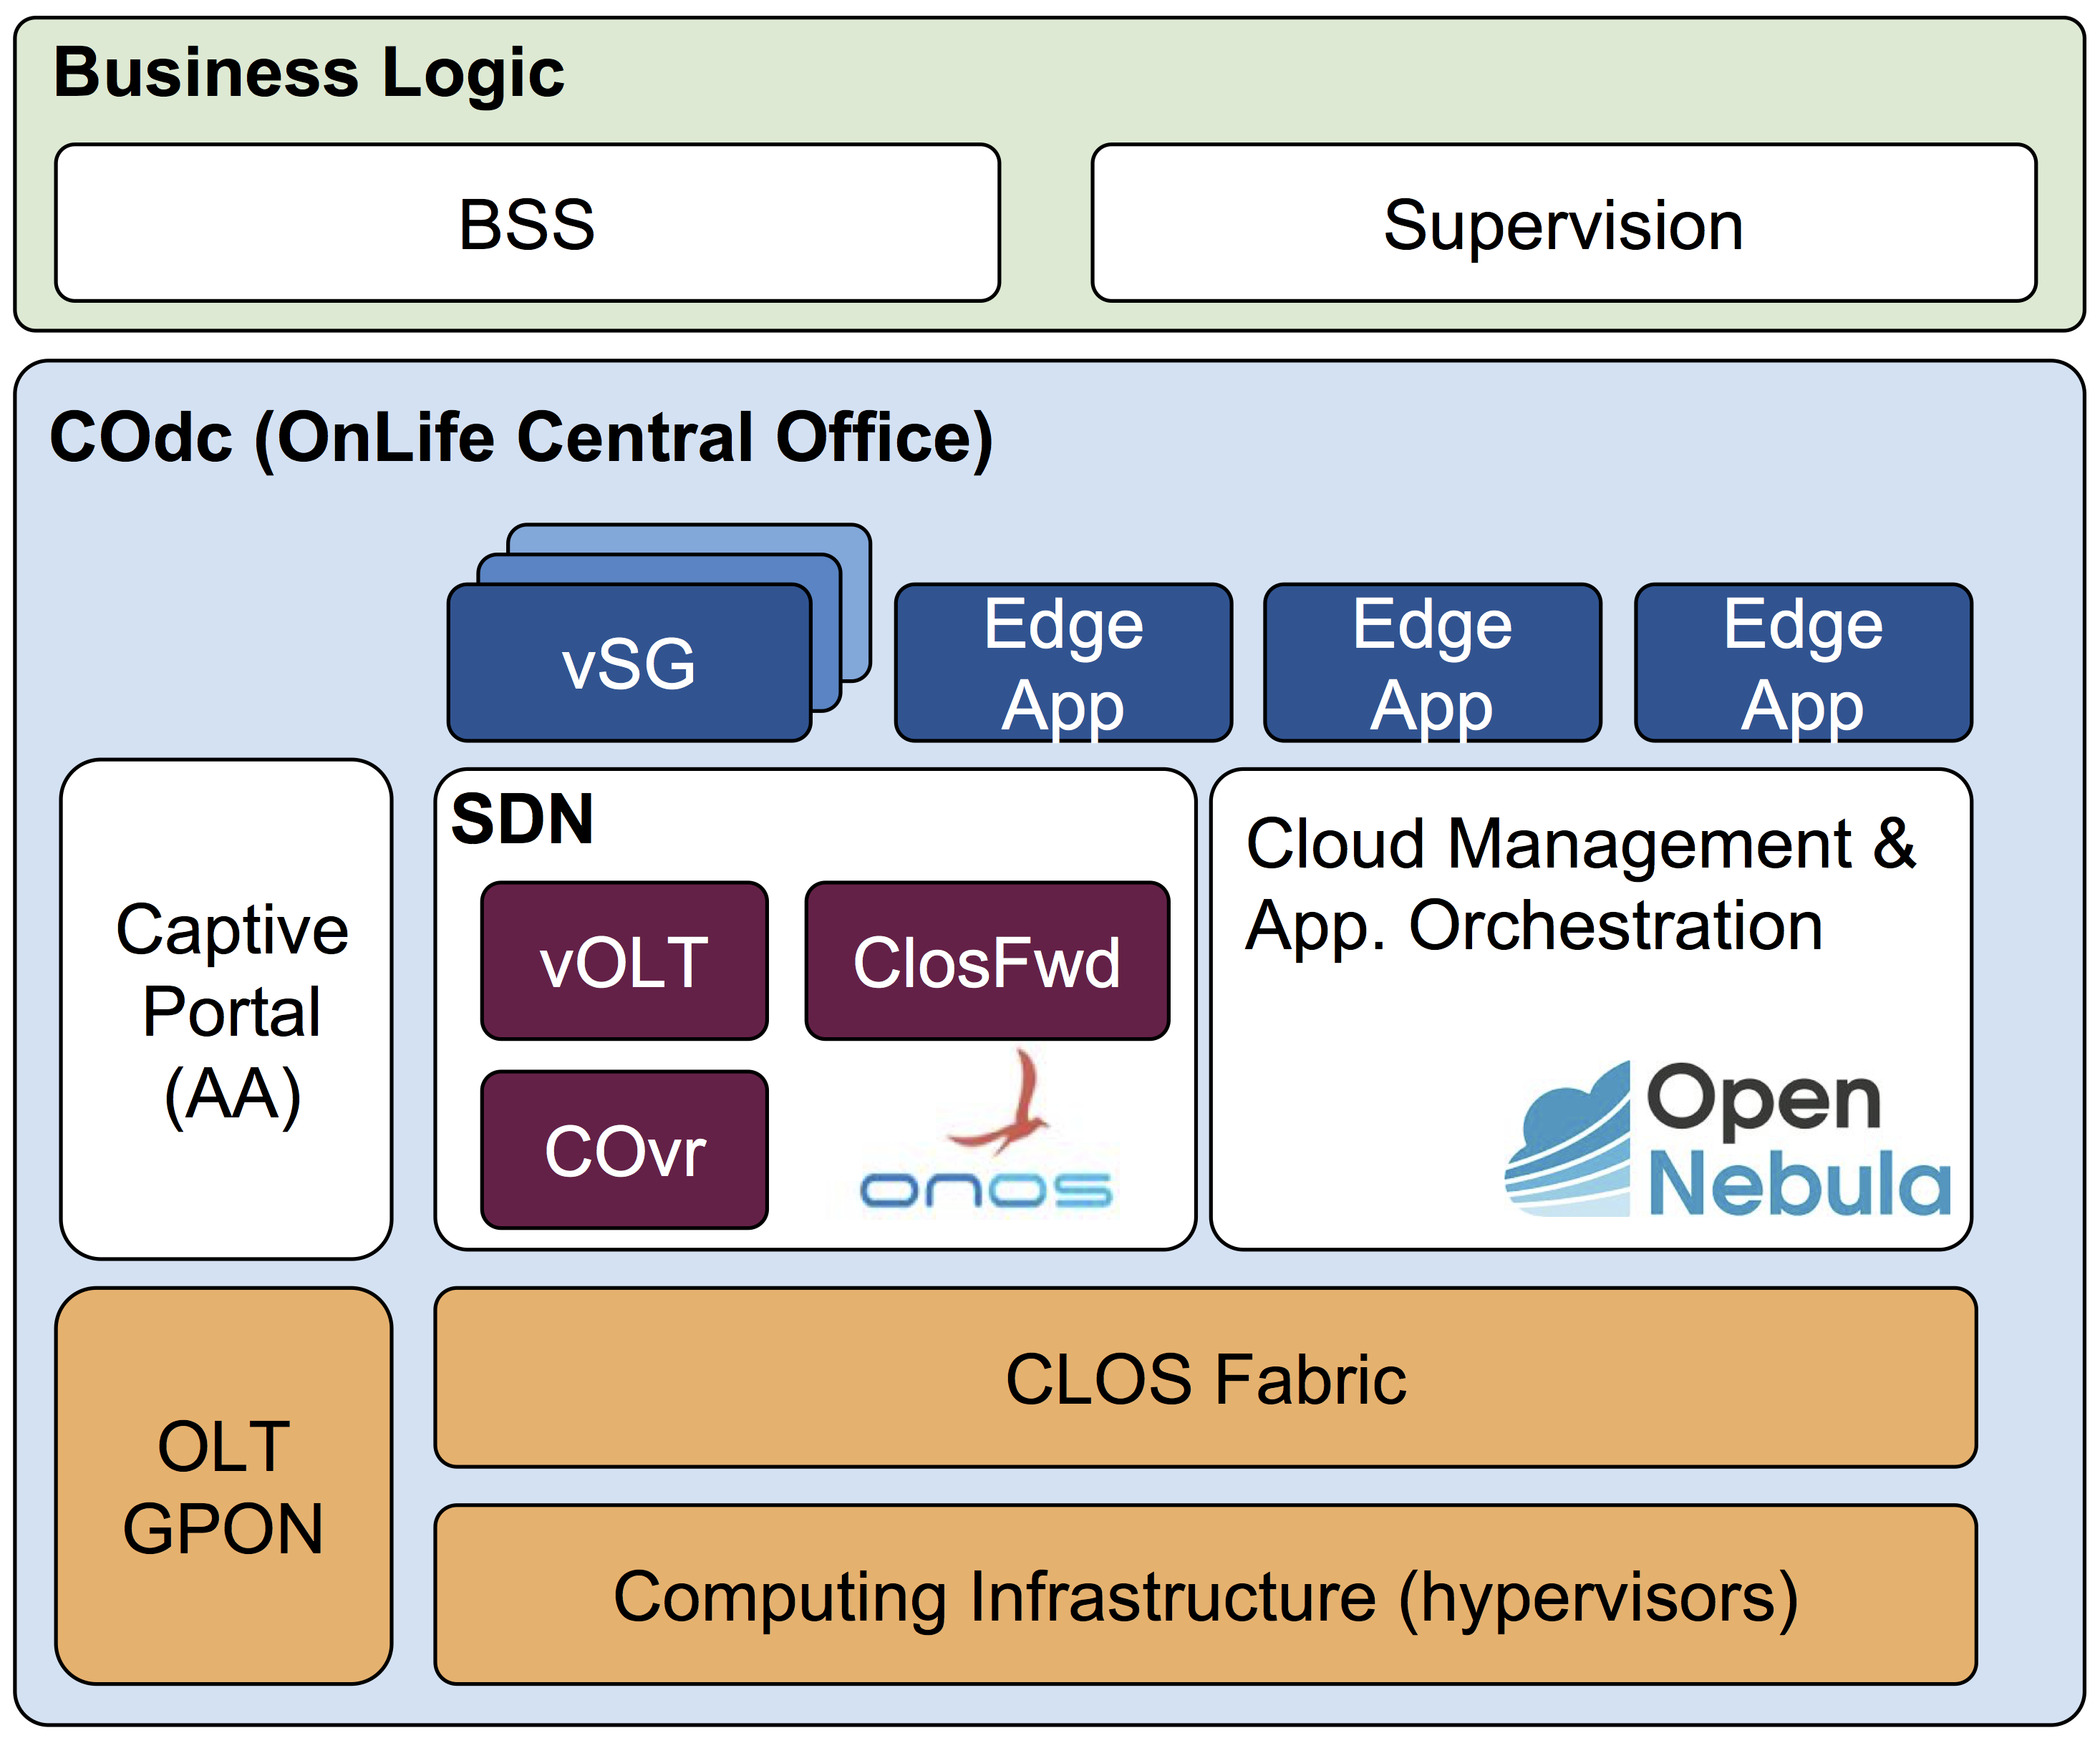
\includegraphics[width=6.5in]{figures/opennebula_edge.png}
~\caption{Telefonica Onlife project}
\label{figure2.3}
\end{figure}

\newpage
\subsubsection{OneEdge}

An OpenNebula distribution that fits into edge computins i OneEdge. This distributed cloud management platform aggregates on-demand cloud resources across multiple edge locations to enable innovate and low-latency next-generation services. ~\cite{onedge}

The main principles of OneEdge are:
\begin{itemize}
    \item Backward compatibility with existing VM \& container appliances
    \item Leverage upcoming ecosystem of hyperscale and edge clouds
    \item Easily combine centralized cloud resources with edge resources
    \item Reuse proven cloud management capabilities
    \item An open-source solution with a growing open ecosystem
\end{itemize}

All these features make OneEdge an interesting option when installing an open source platform int he field of edge computing.

\newpage
\subsection{AWS}
\label{makereference2.3.3}


Amazon Web Services is the main company speaking about cloud services nowadays. Basically Amazon is the principal election when it comes to the public cloud.
This large sized company has a huge amount of products/services and they even have an IoT/Edge computing section.

AWS Outposts ~\cite{aws_outpost} is a fully managed service that extends the whole AWS ecosystem, this new service provided by Amazon can be set forth in a on-premises facility and combine it with public cloud to generate an hybrid experience.

AWS Outpost is ideal for workloading that requires a low latency access and local data processing, in other words, it's suitable for edge computing.

\begin{figure}[h]%t=top, b=bottom, h=here
% \centering
    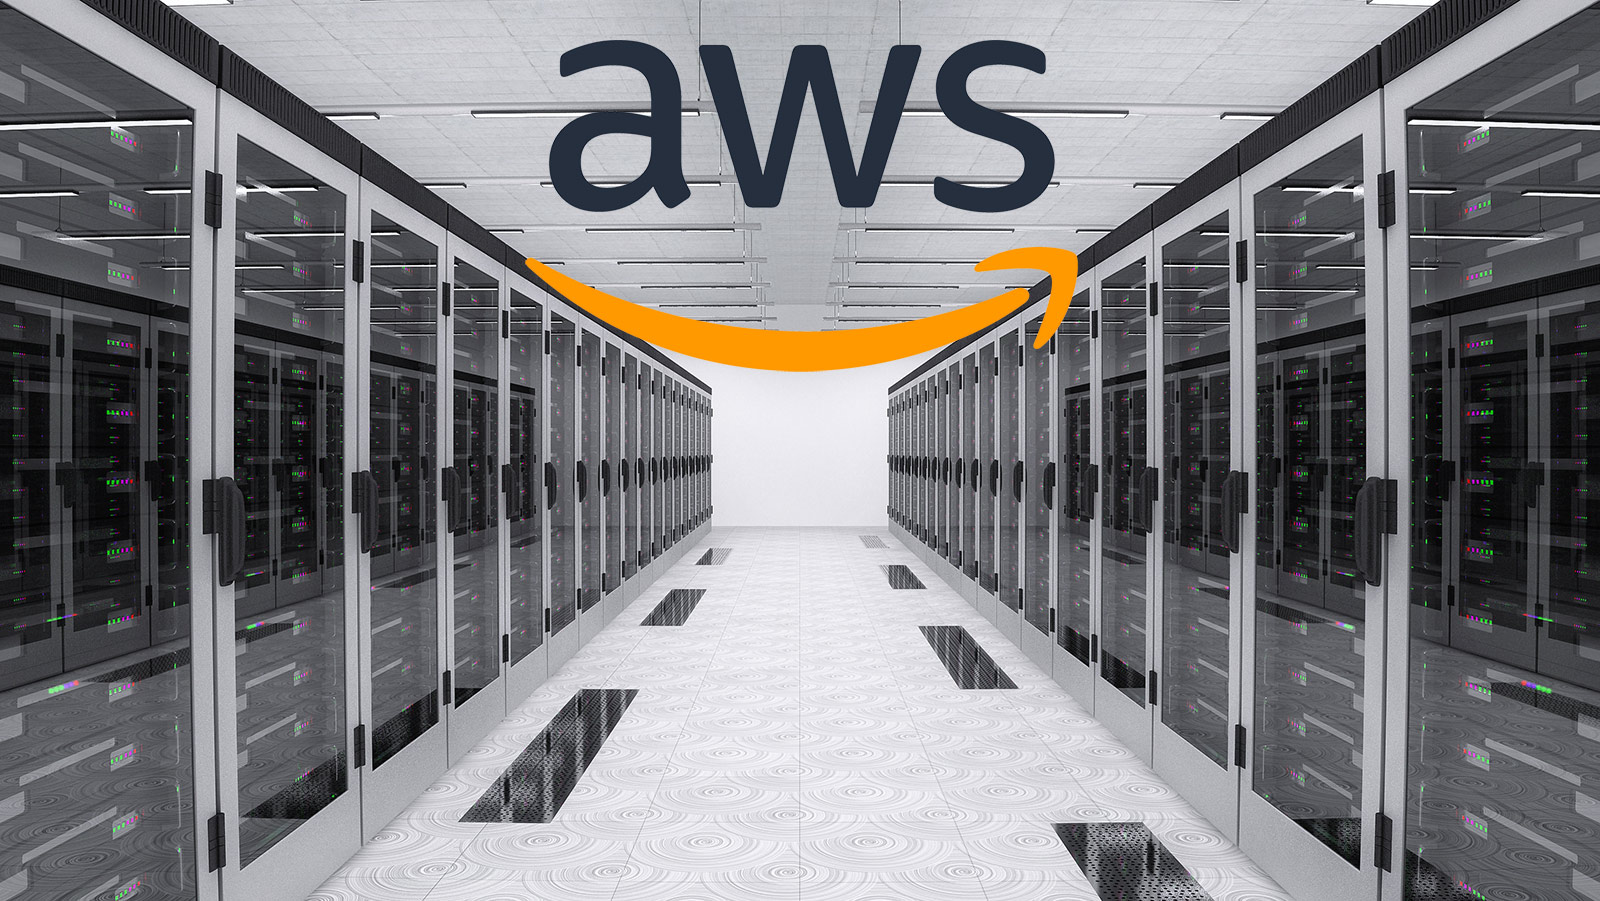
\includegraphics[width=6.5in]{figures/aws_outpost.jpg}
~\caption{AWS Outpost}
\label{figure2.3}
\end{figure}